\subsection{Introducción}

En este ejercicio se implementa un sistema de control para un tanque de agua, el cual cuenta con dos sensores, siendo estos I y S, los cuales indican si el tanque está lleno, por la mitad o vacío. Las condiciones de diseño son las siguientes:
\begin{itemize}
\item Cuando está vacío (I = 0, S = 0) se prenden las dos bombas $B_0 \ y \ B_1$.
\item Cuando se encuentra lleno (I = 1, S = 1) se apagan las bombas.
\item Cuando está por la mitad (I = 1, S = 0) se activa una sola bomba, pero estas se alternan entre sí al establecer cual trabaja.
\end{itemize}

\subsection{Análisis del sistema}
Las limitaciones previamente mencionadas se corresponden con la siguiente tabla de verdad:
\begin{table}[H]
\centering
\begin{tabular}{cccc}
\hline
\textbf{I}              & \textbf{S}             & \textbf{$B_1$}         & \textbf{$B_2$} \\ \hline
0                       & 0                      & 1                      & 1              \\ 
0                       & 1                      & x                      & x              \\ 
1                       & 0                      & \multicolumn{2}{c}{Alternado}          \\ 
\multicolumn{1}{l}{1} & \multicolumn{1}{l}{1} & \multicolumn{1}{l}{0} & 0              \\ \hline
\end{tabular}
\caption{Tabla de verdad del sistema.}
\end{table}

A partir de lo expuesto previamente, se diseña la siguiente FSM.
\begin{figure}[H]
	\centering
	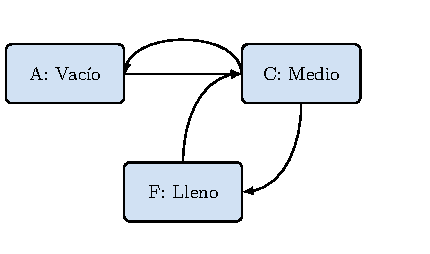
\includegraphics[width=0.5\textwidth, page = 1]{ImagenesEjercicio1/FSM1.pdf}
	\caption{Finite State Machine.}
	\label{fig:fsm}
\end{figure}

Con lo presentado en la Figura (\ref{fig:fsm}), se confecciona una tabla de transiciones.
\begin{table}[H]
\centering
\begin{tabular}{ccccccc}
\hline
\multirow{3}{*}{Estado actual} & \multicolumn{4}{c}{Próximo estado} & \multicolumn{2}{c}{Salida} \\
 & I-S & I-S & I-S & I-S & Ambos & Toggle \\
 & \multicolumn{1}{l}{0-0} & \multicolumn{1}{l}{0-1} & \multicolumn{1}{l}{1-0} & \multicolumn{1}{l}{1-1} & \multicolumn{1}{l}{} & \multicolumn{1}{l}{} \\
 \hline
A & X & X & B & X & 1 & 0 \\
B & A & X & X & C & 0 & 1 \\
\hline
\end{tabular}
\caption{Tabla de transiciones del sistema.}
\label{tab:estados}
\end{table}

A partir de la Tabla (\ref{tab:estados}) y la Figura (\ref{fig:fsm}) se puede llegar a la siguiente tabla, donde $y_1$ e $y_2$ representan la salida de los flip-flops, mientras que $Y_1$ e $Y_2$ la entrada de los mismos.
\begin{table}[H]
\centering
\begin{tabular}{cccccccc}
\hline
\multirow{3}{*}{Estado actual} & Codificación & \multicolumn{4}{c}{Próximo estado} & \multicolumn{2}{c}{Salida} \\
 & $y_2 - y_1$ & \begin{tabular}[c]{@{}c@{}}$Y_2 - Y_1$\\ I-S\end{tabular} & \begin{tabular}[c]{@{}c@{}}$Y_2 - Y_1$\\ I-S\end{tabular} & \begin{tabular}[c]{@{}c@{}}$Y_2 - Y_1$\\ I-S\end{tabular} & \begin{tabular}[c]{@{}c@{}}$Y_2 - Y_1$\\ I-S\end{tabular} & Ambos & Toggle \\
\hline
 &  & 0-0 & 0-1 & 1-0 & 1-1 &  &  \\
A & 00 & X & X & 01 & X & 1 & 0 \\
B & 01 & 00 & X & X & 11 & 0 & 1 \\
C & 10 & X & X & 01 & X & 0 & 0 \\
D & 11 & X & X & X & X & X & X	\\
\hline
\end{tabular}
\end{table}

Se destaca que la variable ``Ambos'' hace referencia a estado en el cual se deben prender ambas bombas, mientras que la variable ``Toggle'' a cuando debe prenderse una sola e intercambiar.

Luego, se prosigue a resolver los mapas de Karnaugh para cada variable:

\begin{figure}[H]
\centering
\begin{subfigure}{.49\textwidth}
\centering
	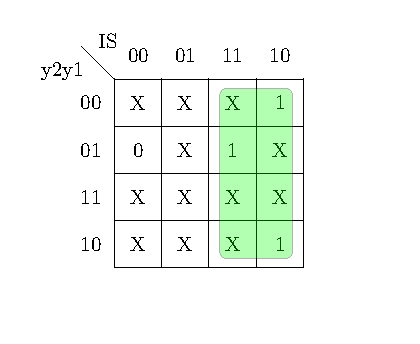
\includegraphics[width=0.7\textwidth]{ImagenesEjercicio1/Mapa1.pdf}
	\caption{Tabla de Karnaugh para $Y_1$.}
	\label{fig:fsm1}
\end{subfigure}
\begin{subfigure}{.49\textwidth}
\centering
	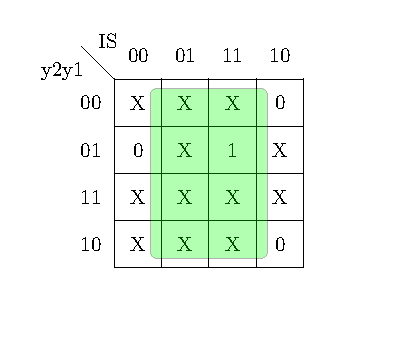
\includegraphics[width=0.7\textwidth]{ImagenesEjercicio1/Mapa2.pdf}
	\caption{Tabla de Karnaugh para $Y_2$.}
	\label{fig:fsm2}
\end{subfigure} \\
\begin{subfigure}{.49\textwidth}
\centering
	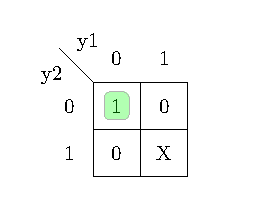
\includegraphics[width=0.5\textwidth]{ImagenesEjercicio1/Mapa3.pdf}
	\caption{Tabla de Karnaugh para ``Ambos''.}
	\label{fig:fsm3}
\end{subfigure}
\begin{subfigure}{.49\textwidth}
\centering
	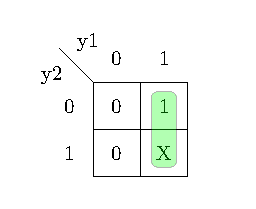
\includegraphics[width=0.5\textwidth]{ImagenesEjercicio1/Mapa4.pdf}
	\caption{Tabla de Karnaugh para ``Toggle''.}
	\label{fig:fsm4}
\end{subfigure}
\caption{Tablas de Karnaugh para cada variable analizada.}
\label{fig:kar}
\end{figure}

A partir de la Figura (\ref{fig:kar}) se derivan las siguientes expresiones:
\begin{equation}
\begin{split}
	Y_1 = & I \\
	Y_2 = & S 
\end{split}
\end{equation}
\begin{equation}
\begin{split}
Ambos = & \ \overline{y_2+y_1} \\
Toggle = & \ y_1
\end{split}
\end{equation}

Luego, se procede a obtener los circuitos para la FSM.
\begin{figure}[H]
\centering
	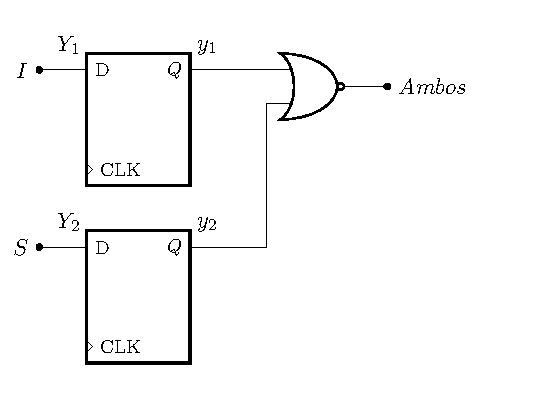
\includegraphics[width=0.6\textwidth, page=1]{ImagenesEjercicio1/Circuitos.pdf}
		\caption{Circuito FSM.}
	\label{fig:fsm1}
\end{figure}

Agregando el siguiente circuito lógico, se implementa la función de Toggle junto a la lógica de salida.
\begin{figure}[H]
	\centering
	\includegraphics[width=0.8\textwidth, page=2]{ImagenesEjercicio1/Circuitos.pdf}
	\caption{Circuito FSM con Toggle.}
	\label{fig:fsm2}
\end{figure}

\subsection{Implementación y mediciones}

Una vez establecidos los circuitos y a partir de ellos, se procedió a implementarlos en PCB:
\begin{figure}[H]
	\centering
	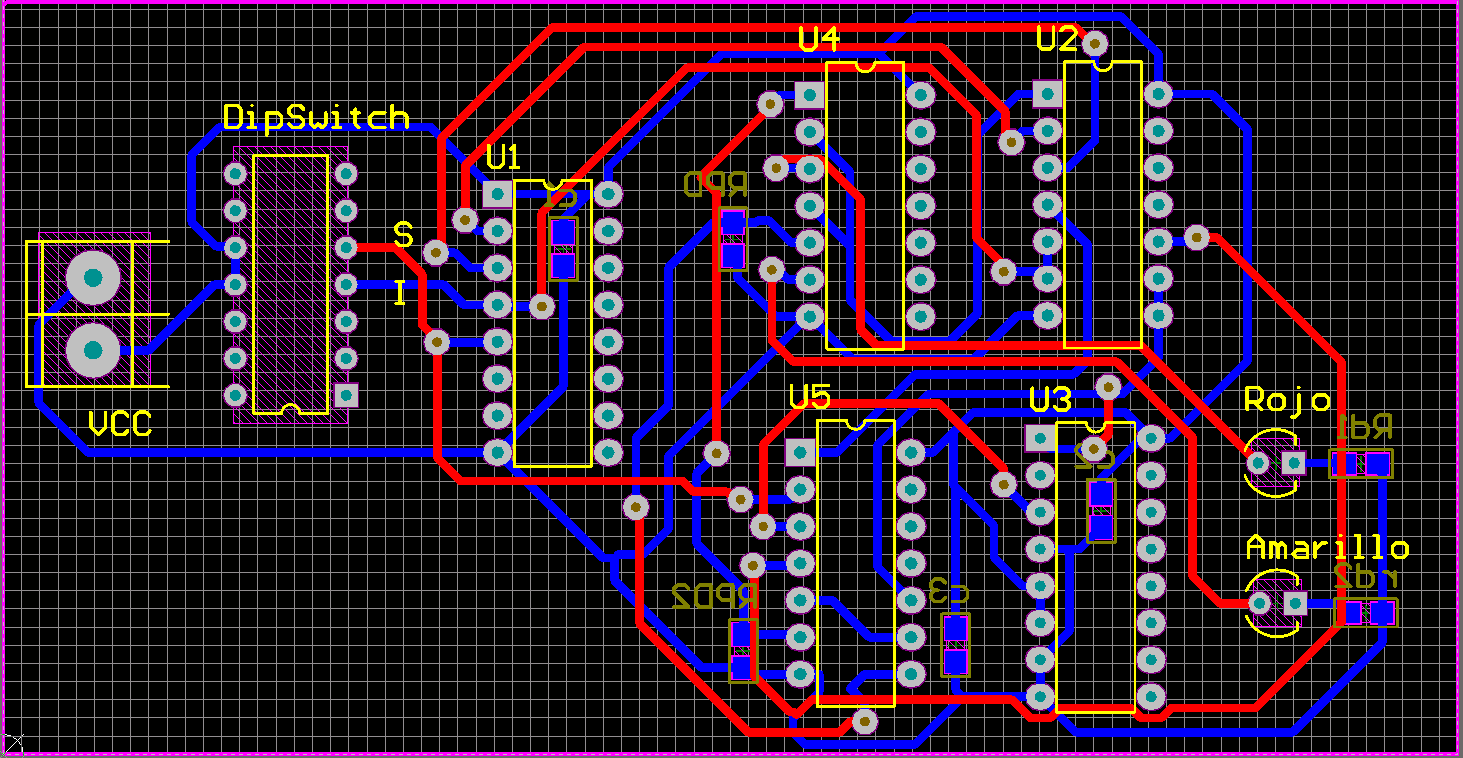
\includegraphics[width=0.7\textwidth]{ImagenesEjercicio1/PCB.PNG}
	\caption{PCB en Altium de los circuitos.}
\end{figure}
\begin{figure}[H]
	\centering
	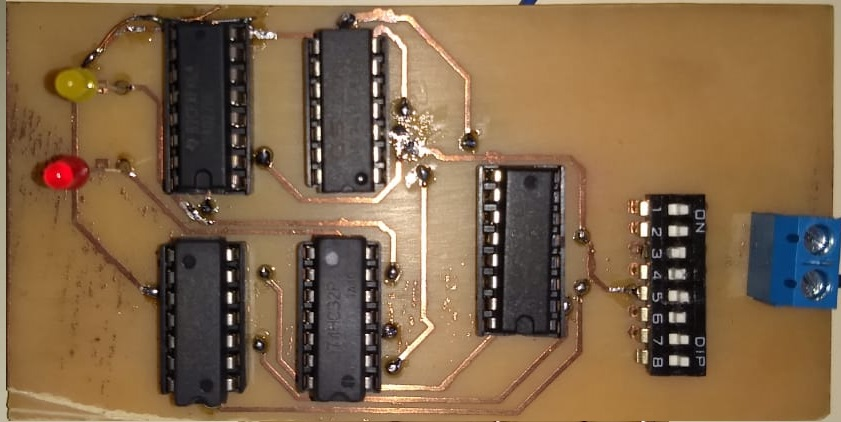
\includegraphics[width=0.8\textwidth]{ImagenesEjercicio1/pcbReal.jpeg}
	\caption{Placa implementada.}
\end{figure}

Finalmente, se procedió a medir los niveles de tensión para las transiciones posibles. A continuación se presentan los resultados.
\begin{figure}[H]
	\centering
	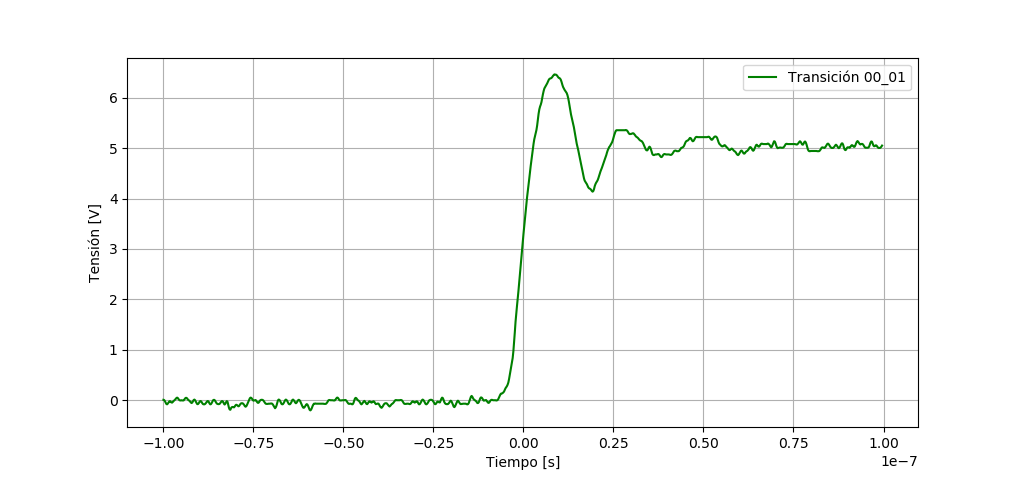
\includegraphics[width=0.8\textwidth]{ImagenesEjercicio1/00-01.PNG}
	\caption{Transición 00-01.}
	\label{fig:0001}
\end{figure}
\begin{figure}[H]
	\centering
	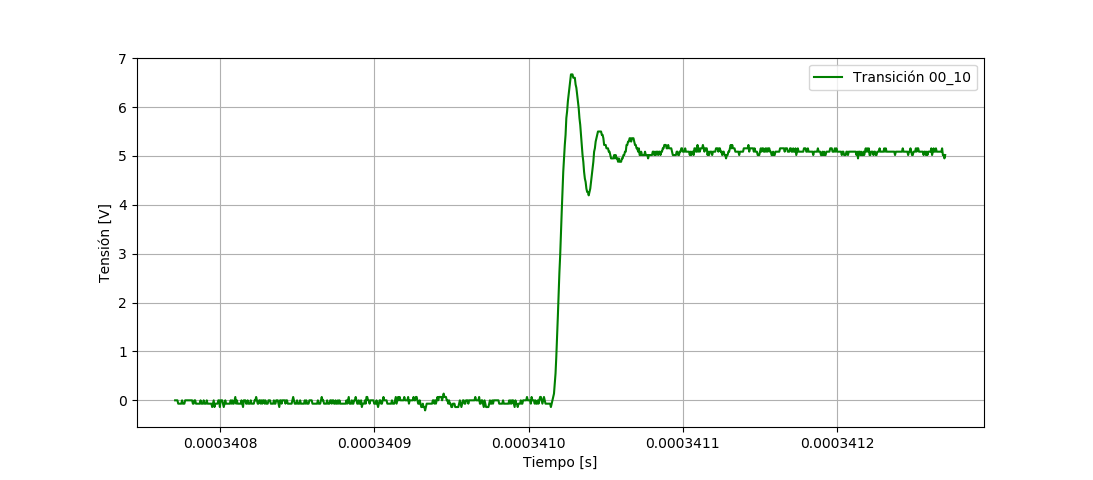
\includegraphics[width=0.8\textwidth]{ImagenesEjercicio1/00-10.PNG}
	\caption{Transición 00-10.}
	\label{fig:0010}
\end{figure}
\begin{figure}[H]
	\centering
	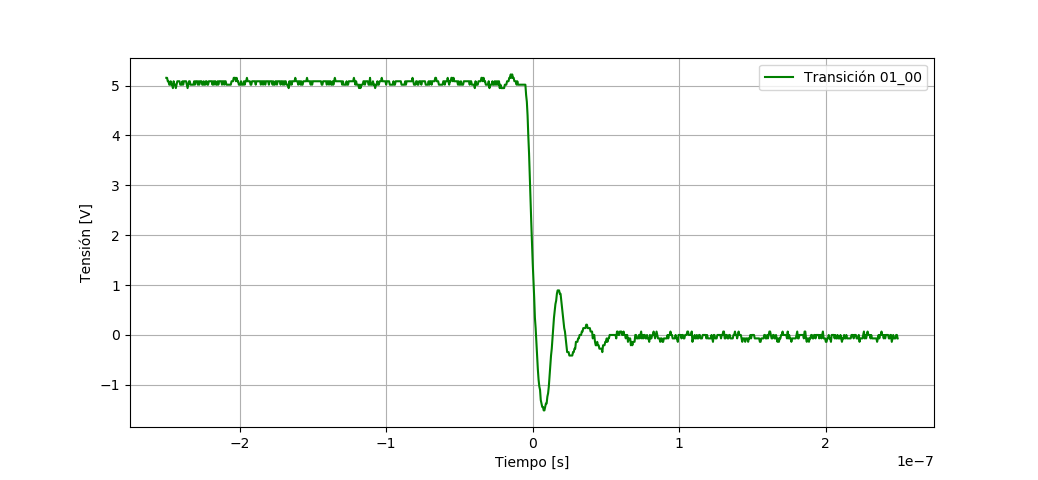
\includegraphics[width=0.8\textwidth]{ImagenesEjercicio1/01-00.PNG}
	\caption{Transición 01-00.}
	\label{fig:0100}
\end{figure}
\begin{figure}[H]
	\centering
	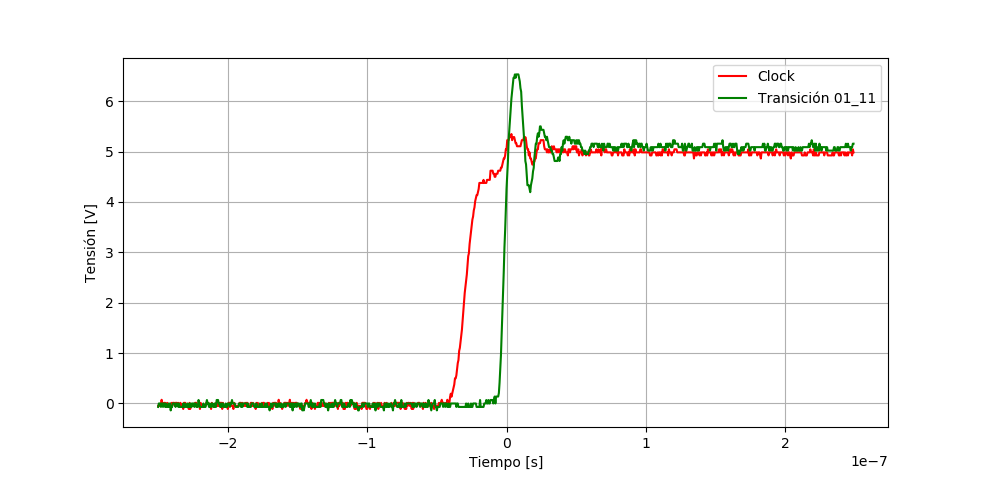
\includegraphics[width=0.8\textwidth]{ImagenesEjercicio1/01-11.PNG}
	\caption{Transición 01-11.}
	\label{fig:0111}
\end{figure}
\begin{figure}[H]
	\centering
	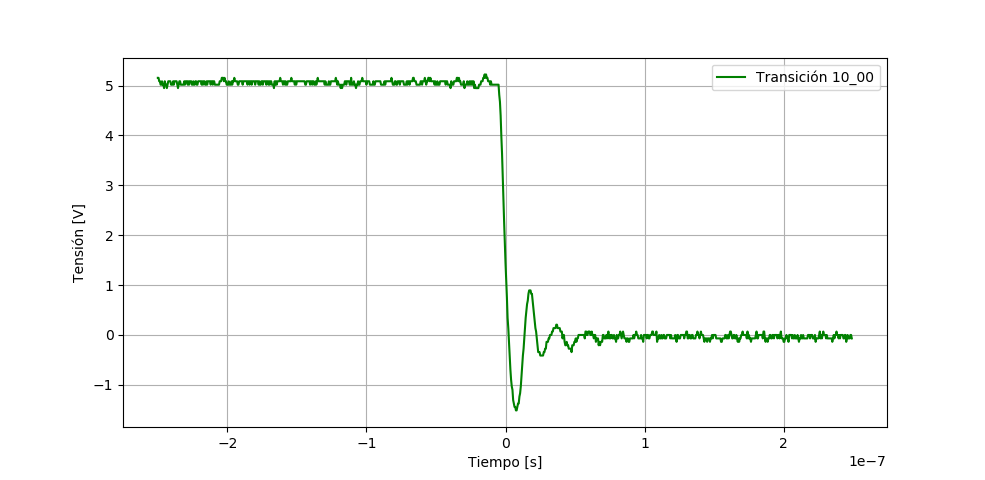
\includegraphics[width=0.8\textwidth]{ImagenesEjercicio1/10-00.PNG}
	\caption{Transición 10-00.}
	\label{fig:1000}
\end{figure}
\begin{figure}[H]
	\centering
	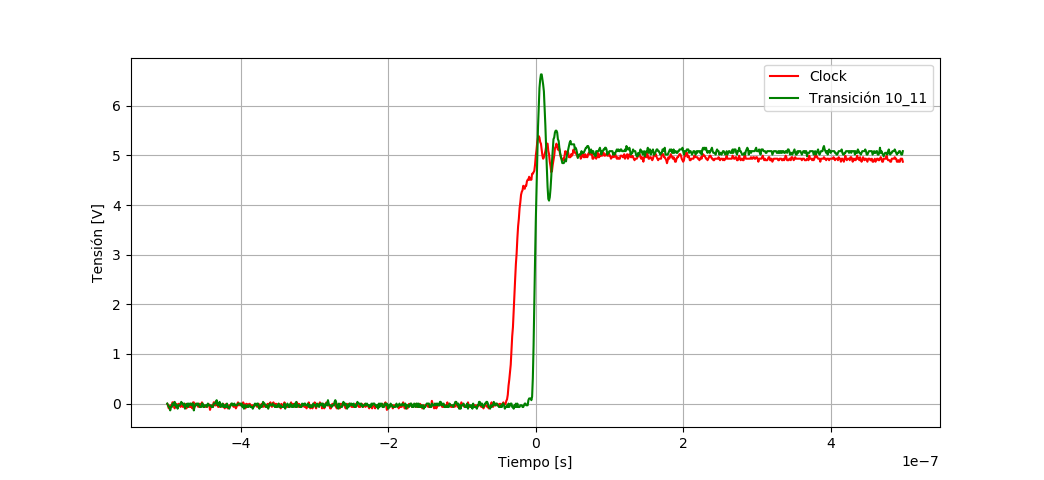
\includegraphics[width=0.8\textwidth]{ImagenesEjercicio1/10-11.PNG}
	\caption{Transición 10-11.}
	\label{fig:1011}
\end{figure}
\begin{figure}[H]
	\centering
	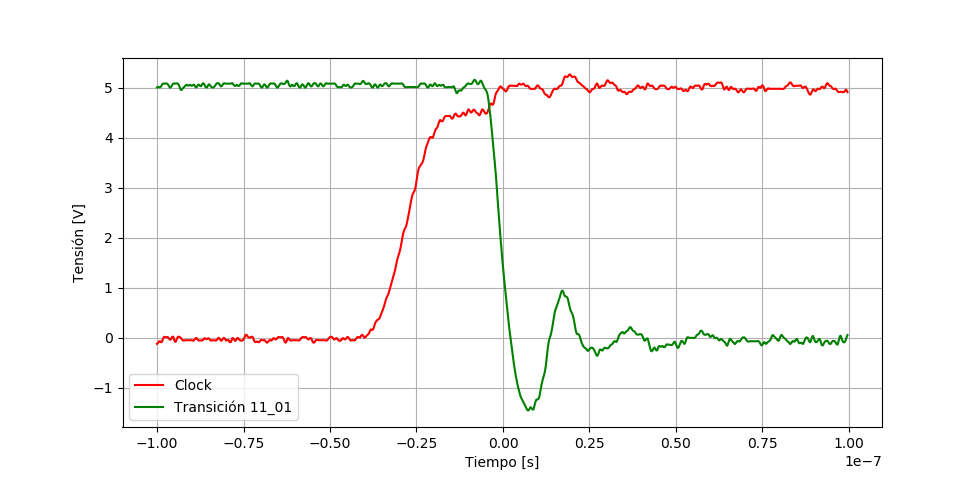
\includegraphics[width=0.8\textwidth]{ImagenesEjercicio1/11-01.PNG}
	\caption{Transición 11-01.}
	\label{fig:1101}
\end{figure}
\begin{figure}[H]
	\centering
	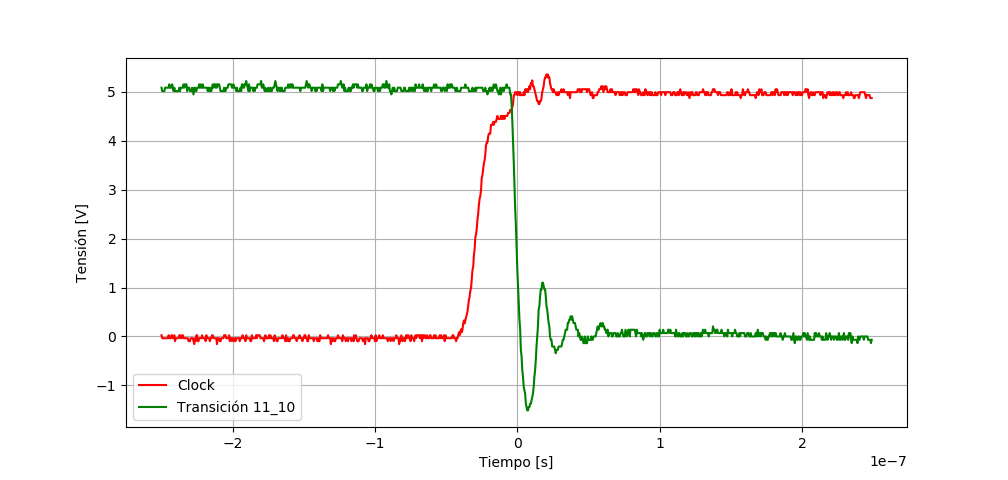
\includegraphics[width=0.8\textwidth]{ImagenesEjercicio1/11-10.PNG}
	\caption{Transición 11-10.}
	\label{fig:1110}
\end{figure}